\documentclass[preprint,12pt]{elsarticle}

\usepackage{amsmath}
\usepackage{amssymb}
\usepackage{booktabs}
\usepackage{graphicx}
\usepackage{float}

\journal{Infrared Physics \& Technology}

\newcommand{\cmark}{\checkmark}
\newcommand{\xmark}{--}

\begin{document}

\begin{frontmatter}

\title{UAV-TAlign-12K: Benchmarking Scene-Level Reliability in\\ Cross-FOV UAV Infrared-Visible Alignment}

\author[anon]{Anonymous Authors}
\affiliation[anon]{organization={Anonymous submission}}

\begin{abstract}
Cross-field-of-view infrared-visible alignment is a core capability for UAV inspection, nighttime
sensing, and multimodal scene understanding. We introduce UAV-TAlign-12K, a benchmark-scale
collection of 6,039 synchronized RGB-infrared pairs acquired across 15 industrial and natural
scenes, together with an integrity-checked 6,037-pair evaluation split. The benchmark organizes
evaluation at three complementary levels: pairwise homography evidence, scene-scale consensus,
and reliability--coverage operating analysis. Seven representative methods span classical
keypoint pipelines, infrared-visible-specific matching, and modern dense or learned matchers.
Pairwise evidence is broadly available: RIFT2, RoMa, and raw MINIMA produce homographies for all
6,037 evaluated pairs, while LoFTR and XoFTR exceed 99\% availability. Building on this evidence,
UAV-TAlign combines progressive evidence scheduling, geometry-calibrated frame weighting, robust
scene consensus, and cross-modal quality verification. It estimates transforms for all 15 scenes
and identifies nine high-confidence alignment products at the canonical operating point, covering
74.4\% of the evaluated pairs. Five-fold leave-frame-out analysis yields a 1.39-pixel median
scene-consensus drift, and controlled translation, rotation, and scale perturbations produce
monotonic degradation of the joint quality signal. UAV-TAlign-12K establishes a reproducible
foundation for benchmark-scale, confidence-aware UAV infrared-visible alignment.
\end{abstract}

\begin{highlights}
\item UAV-TAlign-12K offers 6,039 synchronized cross-FOV RGB-infrared pairs.
\item Seven baselines reveal broadly available pairwise homography evidence.
\item UAV-TAlign yields 15 scene transforms and nine high-confidence products.
\item Resampling and controlled perturbations validate the operating protocol.
\end{highlights}

\begin{keyword}
infrared-visible dataset \sep UAV imagery \sep multimodal registration \sep alignment benchmark \sep scene-level reliability
\end{keyword}

\end{frontmatter}

% !TEX root = ../paper.tex

\section{Introduction}

Infrared-visible alignment is becoming a foundational capability for UAV inspection, monitoring,
and nighttime multimodal perception. Visible imagery provides semantic and structural detail,
while infrared thermal imagery remains informative under illumination changes, smoke, haze, and
low-light conditions. This complementarity has driven progress across multispectral pedestrian
perception, thermal object detection, visible-thermal tracking, and UAV multimodal sensing
\cite{hwang2015kaist,flir2018thermal,jia2021llvip,liu2022tardal,sun2022dronevehicle,zhang2022vtuav,li2022lasher,jiang2023antiuav}.
For these systems to operate as fused sensors rather than separate streams, however, RGB and
thermal observations must be aligned reliably at the scene level.

Real UAV infrared-visible alignment is substantially more demanding than standard same-view image
matching. Aerial platforms introduce viewpoint drift, cross-FOV capture, rolling scale changes, and
cross-resolution sensors; thermal images further introduce low-texture regions, grayscale or
pseudocolor rendering, and strong day/night appearance shifts. These factors make individual
frame-level homographies uneven: some pairs are strongly supported, while others require additional
scene context before they should influence the final transform. The practical question is therefore
not only whether a matcher can produce correspondences for one pair, but whether a system can
decide which scene-level alignment should be trusted.

Recent pairwise matching has advanced rapidly. Transformer, dense, and multimodal matchers such as
LoFTR, LightGlue, DKM, RoMa, XoFTR, and MINIMA have substantially improved correspondence
availability under difficult appearance changes
\cite{sarlin2020superglue,sun2021loftr,chen2022aspanformer,lindenberger2023lightglue,edstedt2023dkm,edstedt2024roma,tuzcuoglu2024xoftr,ren2025minima}.
At the benchmark level, recent UAV visible-infrared alignment studies have also shown that
synthetic transform supervision can support trainable alignment baselines with controlled
geometric metrics \cite{gao2025uavmatch}. UAV-TAlign-12K targets the complementary operating
regime: real captured cross-FOV UAV infrared-visible scenes where the central product is a
retained scene-level transform rather than only a supervised pairwise transform prediction.
Our 12K-scale experiments confirm this progress in the UAV infrared-visible setting: strong
off-the-shelf classical and modern baselines already provide broadly available pairwise homography
evidence on UAV-TAlign-12K. This result creates a concrete
tension: a method can approach saturated pairwise usability while producing only selective
scene-level retention under a strict acceptance rule. Pairwise usability and scene-level
canonical acceptance therefore measure different operating questions and should not be read as the
same success criterion. The key step is to aggregate evidence across a scene, suppress unstable
homographies, and verify whether the final transform should be retained.

Figure~\ref{fig:scene_reliability_principle} illustrates this distinction. Pairwise homographies
can be available for most frames while their support and scene consistency remain uneven; robust
consensus and QA therefore determine whether the resulting scene transform is retained, whereas
the reliability score is used only to rank scenes for operating-profile analysis.

\begin{figure}[t]
\centering
\makebox[\textwidth][c]{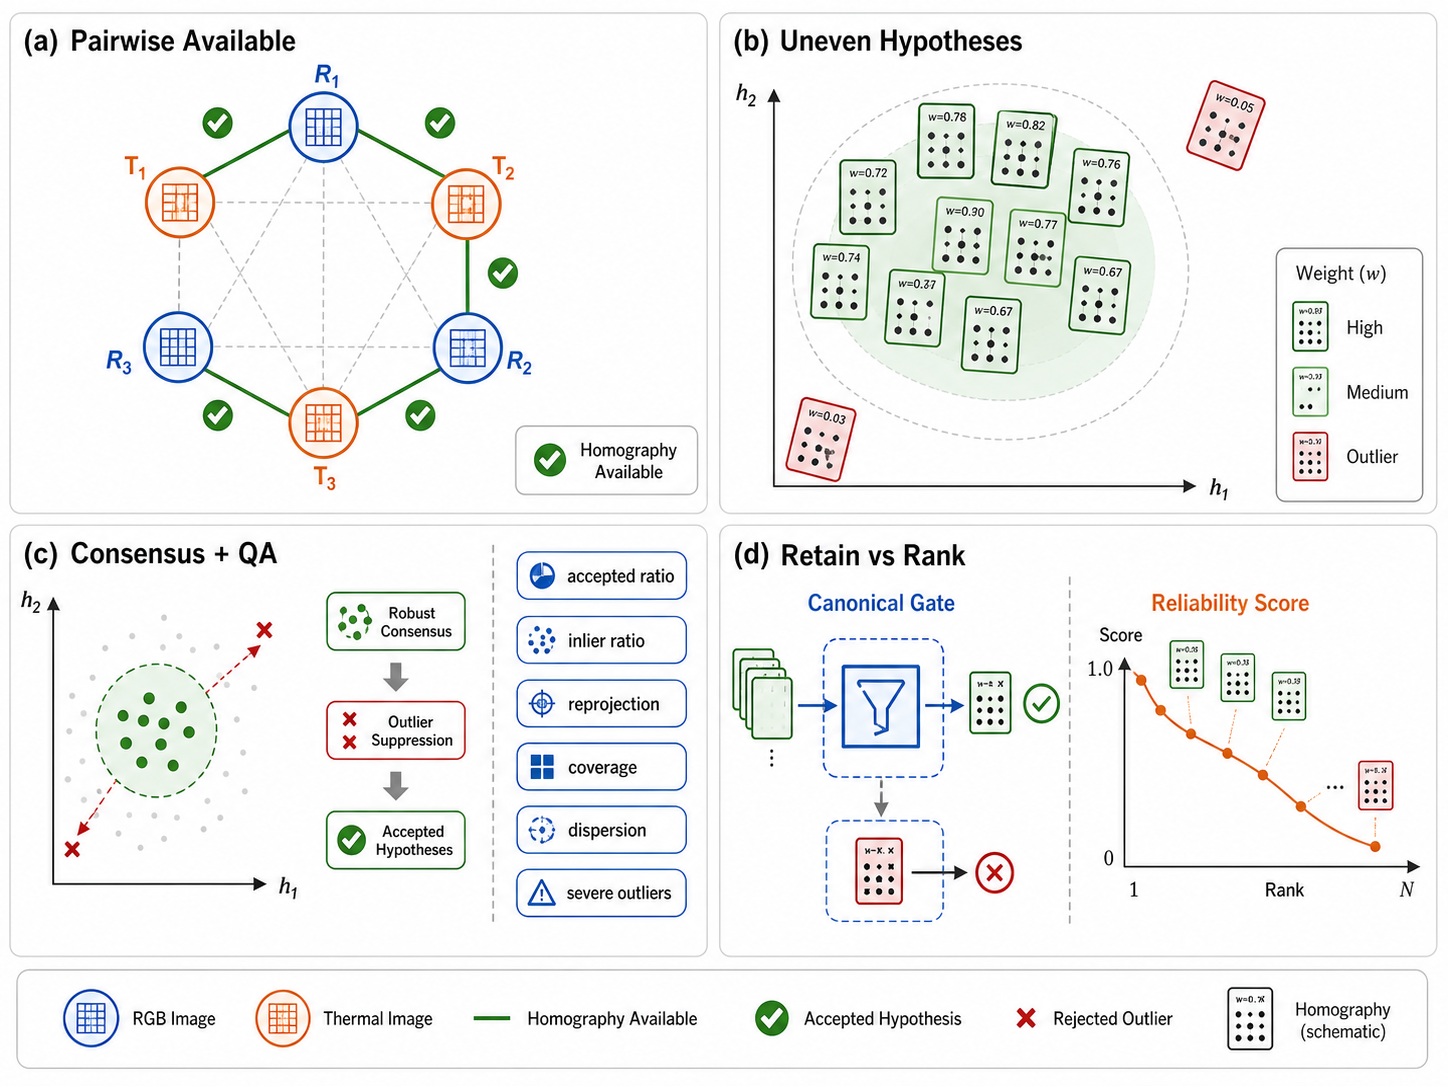
\includegraphics[width=1.05\textwidth]{figures/fig_scene_reliability_principle_image2.png}}
\caption{Principle of scene-level reliability control. Broad pairwise homography availability
does not imply that all frame-level hypotheses are equally trustworthy. UAV-TAlign suppresses
unstable hypotheses, forms a robust scene consensus, and separates the canonical retain/reject
decision from reliability-based ranking.}
\label{fig:scene_reliability_principle}
\end{figure}

This observation motivates a benchmark-first framing with two complementary evaluation questions:
whether a method can produce usable pairwise homography evidence, and whether multi-frame evidence
supports a scene transform that should be retained. Treating these as separate units prevents high
pairwise availability from being interpreted as automatic scene-level reliability.

Our primary contribution is UAV-TAlign-12K, a real-world UAV infrared-visible alignment dataset
with 6,039 candidate pairs and an integrity-checked 6,037-pair evaluation split across 15 scenes.
The collection spans day, night, low-light, grayscale thermal, pseudocolor thermal, and wide,
zoom, and standard UAV views. Its manifest-fixed, label-free protocol evaluates pairwise
homography evidence, canonical scene retention, condition-aware reliability, and risk--coverage
operating profiles. Together, the data and protocol make scene-level alignment reliability
directly studyable under captured cross-FOV UAV conditions.

To instantiate the scene-level benchmark track, we additionally present UAV-TAlign as a reference
alignment method. It operates on top of strong pairwise matchers and uses reliability-guided
evidence selection, robust scene consensus, and QA-aware verification to decide whether a
scene-level transform should be retained. The method contribution is therefore complementary to
the dataset: it provides a reproducible reference implementation for the reliability question
exposed by UAV-TAlign-12K.

Figure~\ref{fig:paper_overview} summarizes the complete paper-level view: UAV-TAlign-12K anchors
pairwise evidence evaluation, UAV-TAlign converts the resulting multi-frame evidence into a
reliability-controlled scene transform, and the protocol reports both canonical retention and the
risk--coverage operating profile.

\begin{figure}[t]
\centering
\makebox[\textwidth][c]{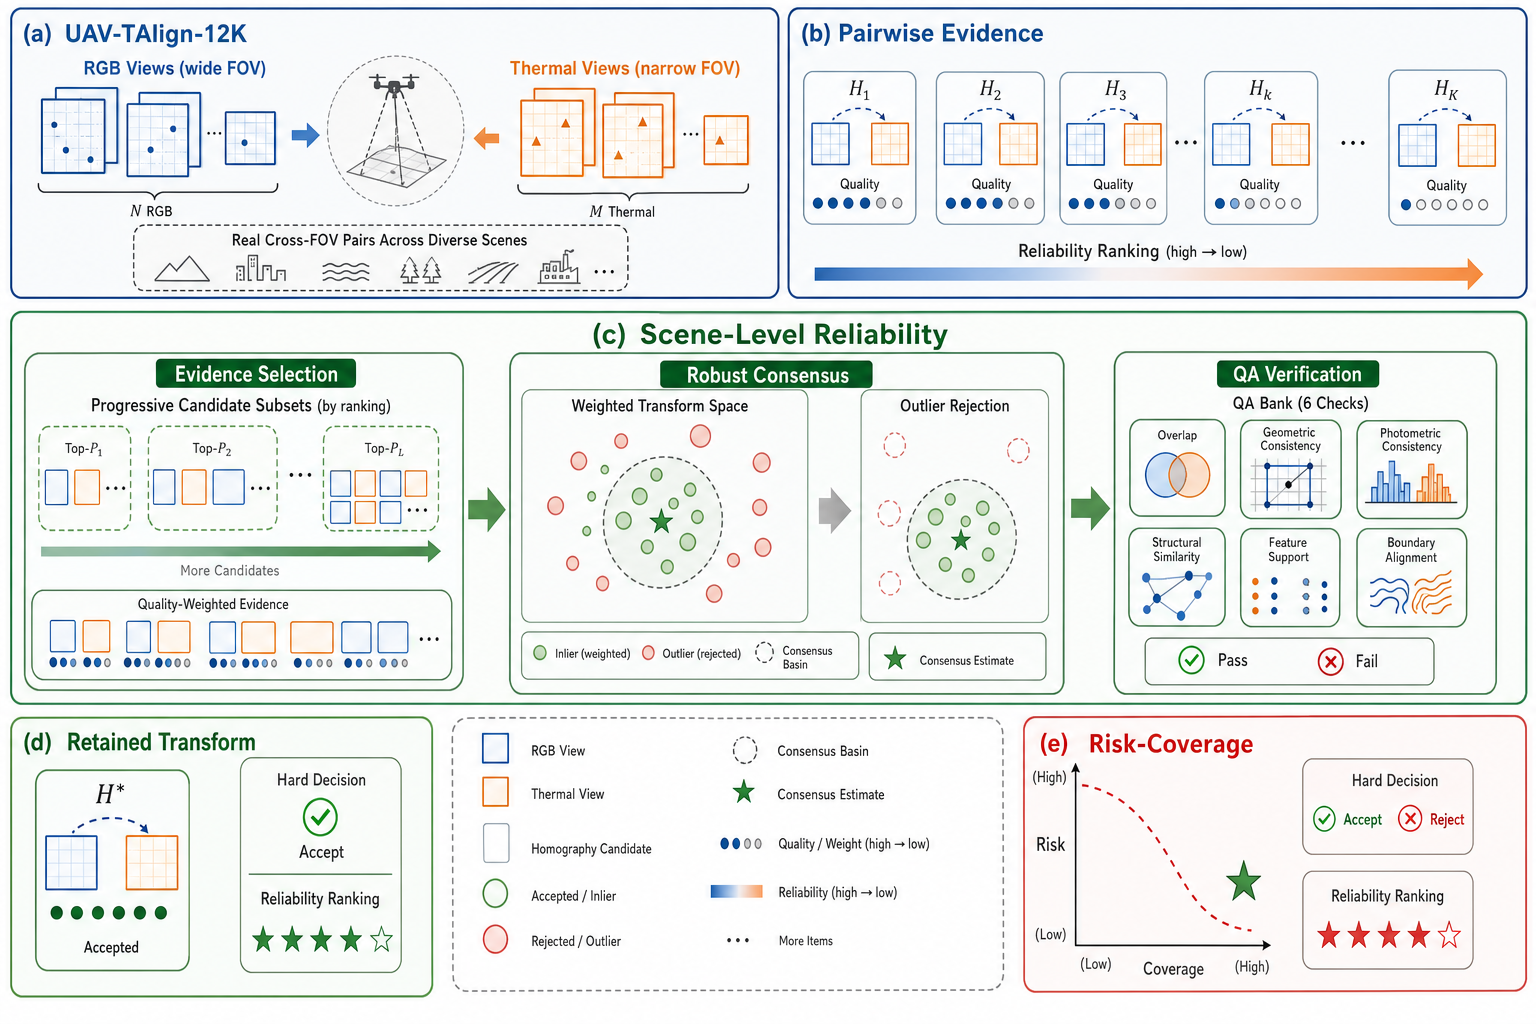
\includegraphics[width=1.15\textwidth]{figures/fig_uav_talign_overview_image2.png}}
\caption{Paper-level overview of UAV-TAlign-12K and UAV-TAlign. The benchmark first measures
pairwise homography evidence, while the reference framework performs scene-level evidence
selection, robust consensus, and QA-aware verification before producing retained alignment
products and reliability--coverage diagnostics.}
\label{fig:paper_overview}
\end{figure}

Our contributions are threefold:
\begin{itemize}
\item We introduce UAV-TAlign-12K, a 6,039-pair real captured cross-FOV UAV infrared-visible
dataset with an integrity-checked 6,037-pair official split across 15 diverse scenes.
\item We establish a manifest-fixed benchmark that separates pairwise homography evidence from
canonical scene-level retention and supports condition-aware and risk--coverage analysis.
\item We provide UAV-TAlign as a scene-level reference method and use classical and modern
off-the-shelf baselines, cumulative ablations, and seed analysis to demonstrate the benchmark's
reliability-centered evaluation capability.
\end{itemize}

% !TEX root = ../paper.tex

\section{Related Work}

\subsection{Cross-Modal Correspondence and Geometric Estimation}

Classical registration combines local feature extraction, descriptor matching, and robust model
estimation. Scale-space, binary, and nonlinear diffusion features provide efficient geometric
references across diverse imaging conditions
\cite{lowe2004sift,bay2008surf,rublee2011orb,leutenegger2011brisk,alcantarilla2012kaze,alcantarilla2013akaze}.
RANSAC and its accuracy-oriented successors remain central to converting noisy correspondences
into geometric models
\cite{fischler1981ransac,hartley2004multiple,barath2019magsac,barath2020magsacpp}.
For infrared-visible imagery, radiation-variation-insensitive constructions such as RIFT improve
descriptor repeatability across modality-specific appearance changes \cite{li2020rift}. These
methods provide an interpretable foundation for separating correspondence quality from downstream
scene aggregation.

Learned correspondence methods have expanded both the robustness and spatial density of pairwise
evidence. Early trainable detectors and descriptors established data-driven local representations
\cite{detone2018superpoint,ono2018lfnet,dusmanu2019d2net,revaud2019r2d2,tyszkiewicz2020disk,germain2020s2dnet,mishchuk2017hardnet,tian2017l2net,tian2019sosnet}.
Graph reasoning, transformers, and dense warp prediction subsequently enabled direct matching
across low texture, repeated structure, and large appearance changes
\cite{sarlin2020superglue,rocco2018ncnet,zhou2021patch2pix,jiang2021cotr,sun2021loftr,chen2022aspanformer,lindenberger2023lightglue,edstedt2023dkm,edstedt2024roma,wang2024efficientloftr,jiang2024omniglue}.
XoFTR and MINIMA further target visible-thermal or broadly multimodal correspondence
\cite{tuzcuoglu2024xoftr,ren2025minima}. UAV-TAlign builds on this progress by treating pairwise
matchers as evidence generators within a scene-scale geometric pipeline.

\subsection{Infrared-Visible Alignment}

Infrared-visible registration spans feature-based matching, direct optimization, and learned
alignment. Radiation-insensitive descriptors address nonlinear cross-modal appearance, while
learned formulations estimate pairwise transforms or dense warps from training data
\cite{li2020rift,chang2017clkn,nie2021udis}. UAV dual-sensor imagery adds cross-resolution optics,
viewpoint displacement, thermal rendering variation, and illumination changes. Registration under
these conditions has motivated dedicated pairwise methods and UAV-specific data resources.

UAVMatch provides synthetic transform supervision and controlled geometric metrics for trainable
UAV alignment \cite{gao2025uavmatch}. ATR-UMMIM contributes 7,969 real UAV
visible--infrared--registered-visible triplets with condition attributes and a semi-automated
pixel-level reference \cite{bin2025atrummim}. UAV-TIRVis provides 80 manually registered aerial
thermal-visible pairs for image-domain evaluation \cite{vasile2025uavtirvis}. UAV-TAlign-12K
complements these resources with a 6,039-pair captured cross-FOV collection and a multi-frame
protocol that connects pairwise homographies, scene consensus, and reliability--coverage operating
analysis.

\subsection{UAV Multimodal Benchmarks and Scene-Scale Evaluation}

Multimodal datasets such as KAIST, FLIR, LLVIP, M3FD, DroneVehicle, VTUAV, LasHeR, and Anti-UAV
have advanced detection, fusion, tracking, and low-light perception
\cite{hwang2015kaist,flir2018thermal,jia2021llvip,liu2022tardal,sun2022dronevehicle,zhang2022vtuav,li2022lasher,jiang2023antiuav}.
Their success demonstrates the value of synchronized visible and infrared sensing. Alignment,
however, requires an explicit geometric product and benefits from evaluation beyond isolated
correspondence counts.

UAV-TAlign-12K defines pairwise, scene, and operating-profile tracks. The
pairwise track measures the availability and support of homography evidence. The scene track
measures how multiple frame estimates form a consensus transform. The operating profile then
orders scene products using fixed, interpretable cross-modal diagnostics. This design makes
scene-scale evidence consolidation directly comparable across classical, infrared-specific, and
modern learned matchers while preserving a common captured-data protocol
\cite{ma2021survey,liao2024survey}.

% !TEX root = ../paper.tex

\section{UAV-TAlign-12K and Evaluation Protocol}

\subsection{Dataset Scope}

UAV-TAlign-12K is a benchmark for real captured UAV infrared-visible alignment. The collection
contains 6,039 synchronized RGB-infrared pairs, corresponding to 12,078 images across 15 scenes.
Its official evaluation split contains 6,037 integrity-checked pairs and 12,074 images. The
collection spans cross-FOV and cross-resolution sensing under day, night, and low-light capture,
grayscale and pseudocolor thermal rendering, and wide, zoom, and standard UAV views.

All journal-scale experiments use the same versioned manifest. UAV-TAlign-1K-Lite is retained as
a fixed development and ablation subset, while UAV-TAlign-12K defines the benchmark-scale
evaluation in this study. The official split comprises 7 day, 5 night, and 3 low-light scenes,
together with 8 grayscale-thermal and 7 pseudocolor-thermal scenes. Paired wide and zoom views
provide controlled cross-FOV comparisons within the substation scene family.

\begin{table}[t]
\caption{Positioning of UAV-TAlign-12K relative to representative infrared-visible and UAV
multimodal resources. UAVMatch denotes the synthetic transform-supervised UAV alignment
benchmark.}
\label{tab:dataset_positioning}
\centering
\resizebox{\textwidth}{!}{
\begin{tabular}{lllll}
\toprule
Resource & Data basis & Alignment signal & Scale & Primary evaluation focus \\
\midrule
KAIST / FLIR / LLVIP / M3FD & Ground or mixed RGB-infrared data & Paired or aligned imagery & Dataset-specific & Detection, fusion, low-light perception \\
DroneVehicle / VTUAV / LasHeR / Anti-UAV & UAV or tracking-centric RGB-infrared data & Task annotations & Dataset-specific & Detection or tracking under multimodal sensing \\
UAVMatch / TGRS~\cite{gao2025uavmatch} & Synthetic transforms from UAV multimodal data & Affine / homography supervision & 81K train / 15K test pairs & Supervised transform regression and geometric metrics \\
ATR-UMMIM~\cite{bin2025atrummim} & Real UAV visible / infrared / registered-visible triplets & Semi-automated pixel-level reference & 7,969 triplets & Pairwise registration accuracy and condition attributes \\
UAV-TIRVis~\cite{vasile2025uavtirvis} & Real UAV thermal-visible imagery & Manual pairwise registration & 80 pairs & Direct image-domain registration quality \\
UAV-TAlign-12K & Real captured cross-FOV UAV infrared-visible data & Multi-frame scene protocol & 6,039 candidate / 6,037 evaluated pairs & Pairwise evidence, scene consensus, and operating coverage \\
\bottomrule
\end{tabular}}
\end{table}

\begin{figure}[t]
\centering
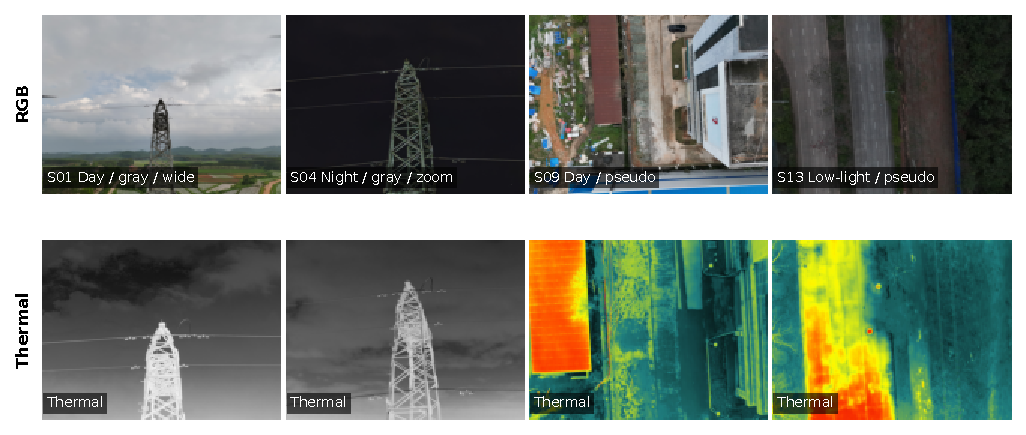
\includegraphics[width=\textwidth]{figures/fig_dataset_examples.pdf}
\caption{Representative UAV-TAlign-12K RGB-infrared pairs spanning illumination, thermal
rendering, and view conditions.}
\label{fig:dataset_examples}
\end{figure}

\subsection{Acquisition and Curation}

UAV-TAlign-12K was acquired between the second half of 2024 and the first half of 2026 across
industrial and natural scenes in southern China. All scenes were captured with the same DJI
Matrice 350 RTK platform and Zenmuse H30T multisensor payload. The integrated payload
automatically synchronized the visible and infrared products, preserving the native cross-sensor
geometry. The flights combined hovering and route-based capture using a registered aircraft, a
CAAC-qualified pilot, and permitted flight areas.

The released streams retain the native H30T acquisition modes. Wide-camera stills are
$4032\!\times\!3024$, zoom-camera stills are $3664\!\times\!2748$, and thermal images are
$1280\!\times\!1024$. In scenes 01 and 02, $3840\!\times\!2160$ still images were triggered while
H30T video recording was active. Scene 07 is a synchronized video-derived sequence sampled at
2 frames per second over one complete orbit around a transmission tower. Grayscale scenes use the
H30T \emph{White Hot} setting, and pseudocolor scenes use the on-device \emph{Hot Iron} palette.

Curation criteria were fixed before algorithm evaluation and covered scene relevance, exposure,
focus, and file integrity. The resulting candidate collection contains 6,039 synchronized pairs;
the integrity audit defines the 6,037-pair official evaluation split. Selection did not use matcher
outputs, alignment estimates, or quality scores.

Release preparation removes embedded metadata and normalizes filenames while preserving image
pixels. RGB and infrared files are linked through their shared H30T capture key, ordered by capture
time and sequence index, and assigned a common six-digit pair identifier. The release applies no
resizing, cropping, rotation, recompression, or image enhancement. Guangxi University owns the
collection, which is prepared for release under the Creative Commons Attribution 4.0 International
license.

\subsection{Dataset Organization}

Each scene has dedicated \texttt{rgb/} and \texttt{thermal/} directories, and paired samples share
the same filename stem. The official manifest records scene identity, pair identity, illumination,
thermal rendering, view type, and scene label. A scene groups frames sharing a site or target
context and acquisition condition. It may represent a continuous sequence or multiple sorties
under the same scene definition. Scene 07 is the documented single-orbit video sequence.

One manifest supports all pairwise, scene, and condition analyses. It also maps every reported
result to its source scene and pair identifier.

\subsection{Multi-Level Evaluation Protocol}

The benchmark defines three complementary tracks. Track A evaluates each of the 6,037 pairs
independently and measures the availability and support of pairwise homography evidence. Track B
aggregates frame estimates into a scene transform and reports the canonical set of high-confidence
scene products. Track C orders scenes with a fixed, interpretable reliability score to construct
coverage-aware operating profiles.

Together, the tracks connect matcher output to deployable scene geometry. Pairwise measurements
characterize evidence generation, scene-level measurements characterize multi-frame consensus,
and the operating profile exposes how product coverage changes with scene quality.

\subsection{Label-Free Scene-Consistency Diagnostics}

The protocol uses label-free relative signals for scalable scene-consistency analysis. The stored
diagnostics compare the optimized transform with its baseline initialization and quantify changes
in cross-modal agreement. They include edge-overlap improvement, gradient-NCC improvement, the
fraction of frames with improved gradient agreement, severe baseline-relative outlier count and
ratio, accepted-frame support, homography dispersion, and robust-rejection ratio.

These signals jointly characterize cross-modal improvement, geometric support, and consensus
stability. The resulting diagnostics support canonical product selection, condition-aware analysis,
and reliability--coverage visualization under a common evaluation interface
\cite{ma2021survey,liao2024survey}.

% !TEX root = ../paper.tex

\section{Method}

\subsection{Problem Formulation}

We study infrared-visible registration as a scene-level alignment task. For each scene, the input is
a set of paired RGB and thermal UAV frames
$S = \{(I_i^R, I_i^T)\}_{i=1}^N$, where viewpoint variation, cross-resolution sensing, thermal
appearance changes, and day/night conditions make individual frame estimates uneven in quality. The
goal is to recover a thermal-to-RGB homography that remains reliable at the scene level, with the
canonical output retained when the evidence satisfies the reliability criterion.

This formulation turns registration from a single best-pair problem into a multi-frame reliability
optimization problem. In our setting, many scenes already contain usable pairwise correspondences,
but the central challenge is to convert uneven frame-level estimates into a transform that is
geometrically stable, internally consistent, and acceptable under a reliability-aware criterion.
For a selected frame pair, the thermal-to-RGB evidence is represented as a homography
$H_i \in \mathbb{R}^{3 \times 3}$ acting on homogeneous image coordinates,
\begin{equation}
\tilde{\mathbf{p}}^{R}_{ij} \sim H_i \tilde{\mathbf{p}}^{T}_{ij},
\qquad
H_i = \arg\min_H \sum_{j \in \mathcal{I}_i}
\rho\!\left(\left\|\pi(H\tilde{\mathbf{p}}^{T}_{ij}) -
\mathbf{p}^{R}_{ij}\right\|_2^2\right),
\label{eq:pairwise_homography}
\end{equation}
where $\mathcal{I}_i$ denotes the inlier set selected by robust fitting, $\pi(\cdot)$ converts a
homogeneous coordinate to image coordinates, and $\rho(\cdot)$ is the robust estimator loss. The
scene-level problem is then to estimate a consensus transform $\bar{H}_S$ from uneven evidence
$\{H_i\}$ and decide whether it should be retained as an alignment product.

\begin{figure}[t]
\centering
\makebox[\textwidth][c]{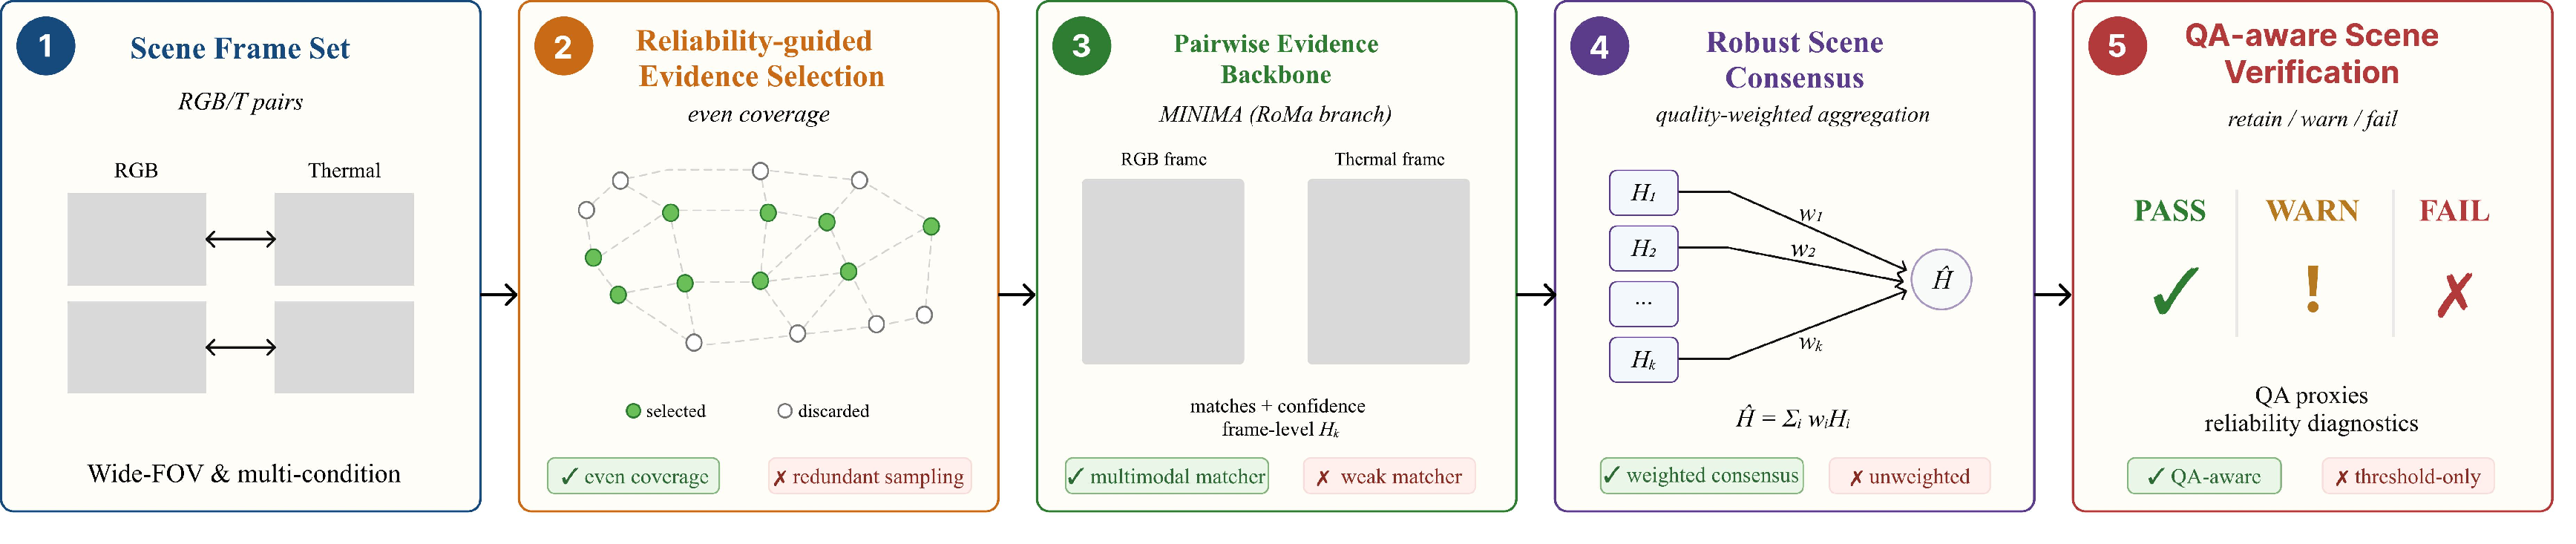
\includegraphics[width=1.35\textwidth]{figures/fig_method_pipeline.pdf}}
\caption{Overview of UAV-TAlign. The framework builds on strong pairwise matching, but
makes the final decision at the scene level through reliability-guided evidence selection, robust
scene consensus, and QA-aware verification.}
\label{fig:method_pipeline}
\end{figure}

\subsection{Pairwise Evidence Backbone}

UAV-TAlign uses a strong off-the-shelf multimodal matcher as its pairwise evidence generator. Our
implementation uses the MINIMA family with the RoMa branch as the default backend, while the
rest of the pipeline remains agnostic to the exact pairwise matcher
\cite{edstedt2024roma,ren2025minima}.

\subsection{Reliability-Guided Evidence Selection}

At the scene level, UAV-TAlign prioritizes the most informative frame evidence before expanding the
support set. It uses a progressive evidence schedule that expands with scene size and can cover all
frames when needed. This reliability-guided policy allows the framework to stop when a compact
subset already yields a stable consensus, while still escalating to broader evidence when the scene
benefits from more support.

Within each stage, representative frames are selected with deterministic evenly distributed
sampling by default. This default policy is used for reproducibility and stable scene coverage. A
random-selection variant is reserved for sensitivity analysis and is reported separately.

\subsection{Quality-Weighted Frame Geometry}

For each selected frame pair, the matcher produces cross-modal correspondences that are filtered
into a frame-level homography estimate. UAV-TAlign evaluates each frame using
standard geometric statistics, including the number of matches, the number of inliers, inlier
ratio, reprojection error, and spatial coverage. A frame enters the global candidate pool only when
it passes a geometry-quality gate on these statistics. The overall geometric treatment remains rooted
in standard homography estimation and robust fitting practice
\cite{hartley2004multiple,fischler1981ransac,barath2019magsac,barath2020magsacpp}.

Beyond a binary accept/reject decision, the pipeline assigns each accepted frame a quality score so
that better-supported homographies receive more influence during scene aggregation. The score is a
weighted combination of inlier ratio, spatial coverage, reprojection quality, matcher confidence,
and inlier count. This keeps the scene-level estimate from being dominated by low-support frames
that only marginally satisfy the frame-level gate.
In normalized form, the frame quality weight is written as
\begin{equation}
q_i =
\alpha_r \phi(r_i) +
\alpha_c \phi(c_i) +
\alpha_e \phi(e_i) +
\alpha_m \phi(m_i) +
\alpha_n \phi(n_i),
\qquad
\sum_k \alpha_k = 1,\ \alpha_k \ge 0,
\label{eq:frame_quality}
\end{equation}
where $r_i$ is inlier ratio, $c_i$ is spatial coverage, $e_i$ is reprojection quality, $m_i$ is
matcher confidence, $n_i$ is inlier support, and $\phi(\cdot)$ maps each diagnostic into a
consistent reliability direction. The weights are fixed by the evaluation protocol and are not
learned from UAV-TAlign-12K.

\subsection{Robust Scene Consensus}

Once enough frame-level homographies have been accepted, UAV-TAlign forms a robust scene consensus.
Homographies are mapped into parameter space, centered with a median reference, and filtered by a
median-absolute-deviation rule to suppress unstable estimates before weighted averaging. The
retained homographies are then combined using the frame quality scores defined above.
Let $\mathbf{h}_i$ be the scale-normalized vector form of $H_i$. The consensus set is
\begin{equation}
\mathcal{C}_S =
\left\{i \in \mathcal{A}_S:
\left\|\mathbf{h}_i - \operatorname{median}_{j \in \mathcal{A}_S}(\mathbf{h}_j)\right\|_1
\le \tau_{\mathrm{mad}}\,\operatorname{MAD}(\{\mathbf{h}_j\}_{j \in \mathcal{A}_S})\right\},
\label{eq:consensus_set}
\end{equation}
where $\mathcal{A}_S$ is the accepted-frame set before robust consensus. The scene transform is
then obtained by quality-weighted aggregation,
\begin{equation}
\bar{\mathbf{h}}_S =
\frac{\sum_{i \in \mathcal{C}_S} q_i \mathbf{h}_i}
{\sum_{i \in \mathcal{C}_S} q_i},
\qquad
\bar{H}_S = \operatorname{mat}(\bar{\mathbf{h}}_S).
\label{eq:scene_consensus}
\end{equation}

The pipeline records stability diagnostics around the aggregate transform, including homography
dispersion relative to the aggregate and the ratio of robustly rejected frame-level estimates.
These diagnostics connect consensus formation with the final QA-aware decision.

\subsection{QA-Aware Scene Verification}

The final decision integrates match availability with scene-level reliability evidence. UAV-TAlign
evaluates the optimized scene-level transform against a label-free QA summary computed on
representative frames. The QA summary uses cross-modal proxy signals such as edge-overlap
improvement, gradient-NCC improvement, the ratio of improved frames, and the count of severe
relative outliers. It also retains scene-level match and stability statistics such as accepted-frame
ratio, mean inlier ratio, mean reprojection error, spatial coverage, dispersion relative to the
aggregate transform, and the robust reject ratio.

The canonical decision uses a baseline-aware verification rule. A scene is retained when
accepted-frame statistics remain strong, the aggregated homography is stable, severe
baseline-relative outliers remain controlled, and the transform improves gradient-based alignment
beyond configured floors. This final verification step gives UAV-TAlign its scene-level character:
the framework prioritizes retained scene-level usability over unconditional scene acceptance.
For operating-profile visualization, the same diagnostics are summarized by a non-trained
reliability score,
\begin{equation}
\begin{aligned}
R(S) ={}&
\beta_a A_S +
\beta_o (1-O_S) +
\beta_d (1-D_S) \\
&+
\beta_e \Delta E_S +
\beta_g \Delta G_S +
\beta_{\gamma} \Gamma_S,
\qquad
\sum_k \beta_k = 1 .
\end{aligned}
\label{eq:reliability_score}
\end{equation}
where $A_S$ is accepted-frame support, $O_S$ is severe baseline-relative outlier ratio, $D_S$ is
homography dispersion, $\Delta E_S$ and $\Delta G_S$ are edge and gradient improvement proxies,
and $\Gamma_S$ collects geometry diagnostics. The strict canonical gate remains a thresholded
decision on the underlying diagnostics,
\begin{equation}
y_S =
\mathbb{1}\!\left[
A_S \ge a_{\min},\ O_S \le o_{\max},\ D_S \le d_{\max},
\Delta G_S \ge g_{\min},\ \Gamma_S \in \mathcal{G}
\right].
\label{eq:canonical_gate}
\end{equation}
Thus $R(S)$ ranks scenes for risk-coverage analysis, while $y_S$ defines the retained canonical
alignment products reported in the main result.

% !TEX root = ../paper.tex

\section{Experimental Setup}

\subsection{Baselines}

We evaluate both classical and learning-based baselines under an explicit off-the-shelf setting.
All learning-based methods use public pretrained weights or public pretrained model interfaces and
are evaluated without training or adaptation on UAV-TAlign-12K. This choice keeps the comparison
focused on practical deployability rather than dataset-specific adaptation.
Unified inference wrappers standardize model loading, image I/O, homography fitting, and output
schemas while preserving the public pretrained baseline parameters and settings.

The baseline suite includes a domain-specific infrared-visible classical method and modern
dense/learned matchers. RIFT2 is evaluated through a Python implementation under a resize-aware
setting. The modern pairwise baselines are Kornia LoFTR (pretrained="outdoor"), RoMa outdoor full,
XoFTR-640, and raw MINIMA. Raw MINIMA uses the MINIMA RoMa branch as a direct pairwise baseline;
reliability-guided evidence selection, robust scene consensus, and QA-aware verification are
activated in the UAV-TAlign full framework
\cite{li2020rift,sun2021loftr,edstedt2024roma,tuzcuoglu2024xoftr,ren2025minima}.

\subsection{Shared Geometric Fitting}

For the pairwise methods, the common downstream step is homography fitting from the predicted
correspondences. After each matcher returns point pairs and optional confidence values, the
shared evaluator estimates a homography with a robust backend and then records a unified outcome
category. This unified post-processing is important because it makes the pairwise baseline
table comparable at the level of usable registration outcomes rather than raw matcher outputs
alone.

The common evaluator uses a robust homography backend across the modern pairwise baselines:
\begin{itemize}
\item robust fitting method: USAC-MAGSAC;
\item reprojection threshold: 3.0;
\item confidence: 0.999;
\item maximum iterations: 10000;
\item spatial coverage grid: $4 \times 4$.
\end{itemize}

RIFT2 is reported as \emph{RIFT2 (Python, resize-aware)}. Its disclosed configuration is
\texttt{max\_dim=1200}, \texttt{npt=2000}, \texttt{patch\_size=64}, Lowe ratio 0.95, and OpenCV
USAC-MAGSAC for downstream homography estimation. We report it as a fixed Python resize-aware
deployment setting for the UAV-TAlign-12K evaluation.

\subsection{Main-Table Baseline Choices}

The main-table baseline choices are as follows. Raw MINIMA uses the MINIMA RoMa backend
with the \texttt{minima\_roma} checkpoint family and the large/full RoMa branch. RoMa uses the
public outdoor full model. XoFTR uses the 640-resolution visible-thermal checkpoint family as the
default main-table setting. Kornia LoFTR (pretrained="outdoor") uses the public pretrained outdoor
model from Kornia.

\subsection{Evaluation Details}

The LoFTR baseline is evaluated under a resize-aware inference setting. The longest image
dimension used for matching is limited to 1600, and automatic mixed precision is disabled. This
deployment setting preserves the public pretrained model while supporting consistent full-subset
evaluation within the fixed deployment budget.

All experiments were run in a Linux Conda environment with Python 3.10,
PyTorch 2.0.1, torchvision 0.15.2, and CUDA 11.8 for the main learned baselines and UAV-TAlign
pipeline. RIFT2 is executed in an independent Python environment. All evaluation outputs are
written to isolated result roots, with raw dataset directories and source trees treated as
read-only inputs during evaluation.

% !TEX root = ../paper.tex

\section{Results}

\subsection{Pairwise Infrared-Visible Homography Evidence}

Pairwise infrared-visible homography evidence is broadly available on UAV-TAlign-12K.
Table~\ref{tab:pairwise_baselines} reports the full 6,037-pair official evaluation split.
Classical keypoint baselines provide useful but less complete pairwise evidence: SIFT and AKAZE
reach 87.08\% and 94.29\% homography availability, respectively. This provides a classical
keypoint reference, while modern dense and learned matchers further improve pairwise availability
under infrared-visible appearance gaps. Raw MINIMA and RoMa produce homographies for all pairs,
while the accepted LoFTR retry and XoFTR remain near-saturated under the same manifest-based
evaluation. This result sharpens the role of UAV-TAlign: once pairwise homography evidence is
broadly available, the main remaining operating question is whether the resulting scene-level
product should be retained.

\begin{table}[t]
\caption{Pairwise infrared-visible homography evidence on UAV-TAlign-12K. Metrics are complementary
diagnostics under the evaluated implementation and deployment settings, and should not be read as
a single absolute ranking. The LoFTR row is reported from the accepted memory-safe retry profile.
LoFTR and XoFTR non-ok cases correspond to insufficient matches, no matches, or homography fitting
failures.}
\label{tab:pairwise_baselines}
\centering
\resizebox{\textwidth}{!}{
\begin{tabular}{llrrrrrr}
\toprule
Method & Category & OK / N $\uparrow$ & H (\%) $\uparrow$ & Inlier Ratio $\uparrow$ & Coverage $\uparrow$ & Median Reproj. $\downarrow$ & Runtime / Pair (s) $\downarrow$ \\
\midrule
SIFT + RANSAC & Classical keypoint & 5257/6037 & 87.08 & 0.242 & 0.627 & 0.000 & 4.421 \\
AKAZE + RANSAC & Classical keypoint & 5692/6037 & 94.29 & 0.160 & 0.730 & 0.105 & 1.103 \\
raw MINIMA & Modern dense / learned & 6037/6037 & \textbf{100.00} & 0.319 & 1.000 & 1.773 & 1.346 \\
RoMa outdoor & Modern dense / learned & 6037/6037 & \textbf{100.00} & 0.328 & 0.997 & 1.741 & 0.929 \\
Kornia LoFTR outdoor (retry) & Modern dense / learned & 5984/6037 & 99.12 & 0.074 & 0.895 & 0.823 & 0.169 \\
XoFTR-640 & Modern dense / learned & 5989/6037 & 99.20 & 0.089 & 0.949 & 1.732 & 0.647 \\
\bottomrule
\end{tabular}}
\end{table}

The classical baselines remain informative reference points, but the modern dense and learned
matchers provide substantially broader usable pairwise support. The LoFTR result is reported with
the accepted resize-aware retry configuration, which enables stable full-subset evaluation under
the fixed memory budget after the original full-resolution run exceeded that budget. These
secondary fitting statistics are therefore most informative when read jointly rather than as a
single absolute ranking.

\subsection{Scene-Level Reference Result}

To instantiate the benchmark's scene-level track, we evaluate UAV-TAlign as the reference method.
High pairwise usability does not automatically imply broad scene retention because the canonical
decision answers a different operating question. UAV-TAlign produces scene-level homographies for
all 15 scenes and retains 9 under the strict canonical reliability gate. This result demonstrates
how UAV-TAlign-12K distinguishes homography availability from retained scene reliability.

\begin{table}[t]
\caption{Strict canonical scene-level result for UAV-TAlign on UAV-TAlign-12K. Arrows indicate the
preferred direction.}
\label{tab:scene_level_main}
\centering
\resizebox{\textwidth}{!}{
\begin{tabular}{llrrrrrr}
\toprule
Method & Eval Unit & H Available $\uparrow$ & Retained Scenes $\uparrow$ & Retention Rate (\%) $\uparrow$ & Pair Coverage (\%) $\uparrow$ & Accepted / Attempted & Accepted Ratio (\%) $\uparrow$ \\
\midrule
UAV-TAlign & 15 scenes & 15/15 & 9/15 & 60.0 & 74.4 & 1491/2304 & 64.7 \\
\bottomrule
\end{tabular}}
\end{table}

\subsection{Condition Breakdown}

Retained alignments show meaningful condition structure across illumination and thermal rendering.
Table~\ref{tab:light_condition} separates condition-level scene retention from accepted-frame
support aggregated over all scenes within each condition. Day scenes retain most frequently and
also provide the strongest accepted-frame support, whereas night scenes are weakest on both axes.
Low-light scenes retain less often than day scenes despite a moderate accepted-frame ratio,
indicating that frame-level support alone does not determine the final scene-level decision.

\begin{table}[t]
\caption{Scene-level reliability breakdown by light condition on UAV-TAlign-12K. Accepted /
attempted aggregates accepted and attempted frames over all scenes within each condition and thus
complements the retained-scene counts.}
\label{tab:light_condition}
\centering
\resizebox{\textwidth}{!}{
\begin{tabular}{lrrrrr}
\toprule
Condition & Scenes & Retained $\uparrow$ & Retention (\%) $\uparrow$ & Accepted / Attempted $\uparrow$ & Accepted Ratio (\%) $\uparrow$ \\
\midrule
Day & 7 & \textbf{5} & \textbf{71.4} & \textbf{1650/2203} & \textbf{74.9} \\
Night & 5 & 3 & 60.0 & 361/890 & 40.6 \\
Low-light & 3 & 1 & 33.3 & 462/754 & 61.3 \\
\bottomrule
\end{tabular}}
\end{table}

\begin{figure}[t]
\centering
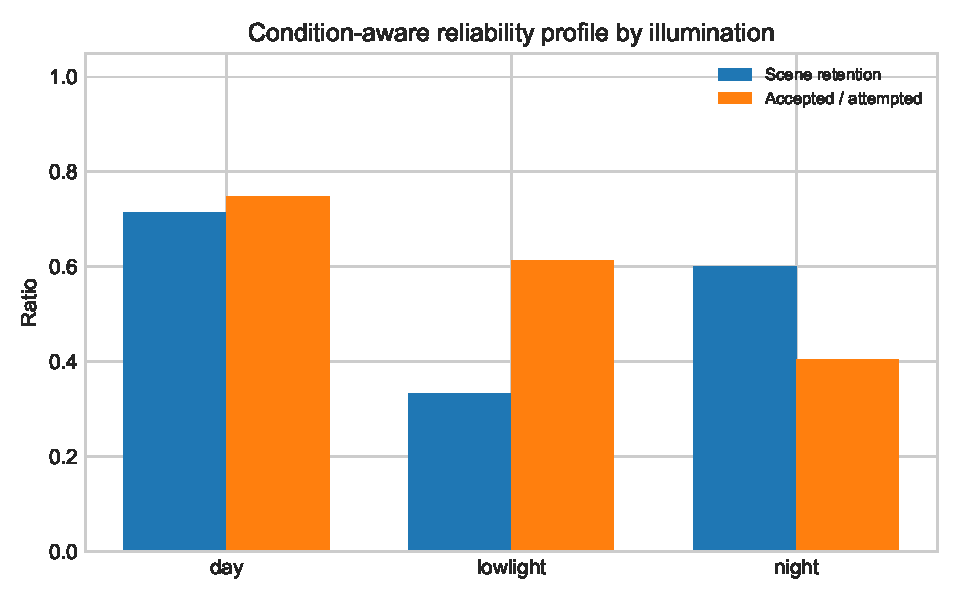
\includegraphics[width=0.78\textwidth]{figures/fig_condition_reliability_profile.pdf}
\caption{Condition-aware reliability profile by illumination. Scene retention and accepted-frame
support summarize complementary aspects of the retained alignment products.}
\label{fig:condition_reliability}
\end{figure}

\subsection{Reliability-Coverage Operating Profile}

The canonical QA gate defines retained alignment products, while the reliability score is used for
ranking, threshold sweep, and operating-profile visualization. The score-ranked top-$K$ subsets and
the canonical retained-scene set are related but not identical. Figure~\ref{fig:risk_coverage}
therefore marks the strict canonical 9/15 operating point explicitly while plotting the
score-ranked reliability--coverage curve.

\begin{figure}[t]
\centering
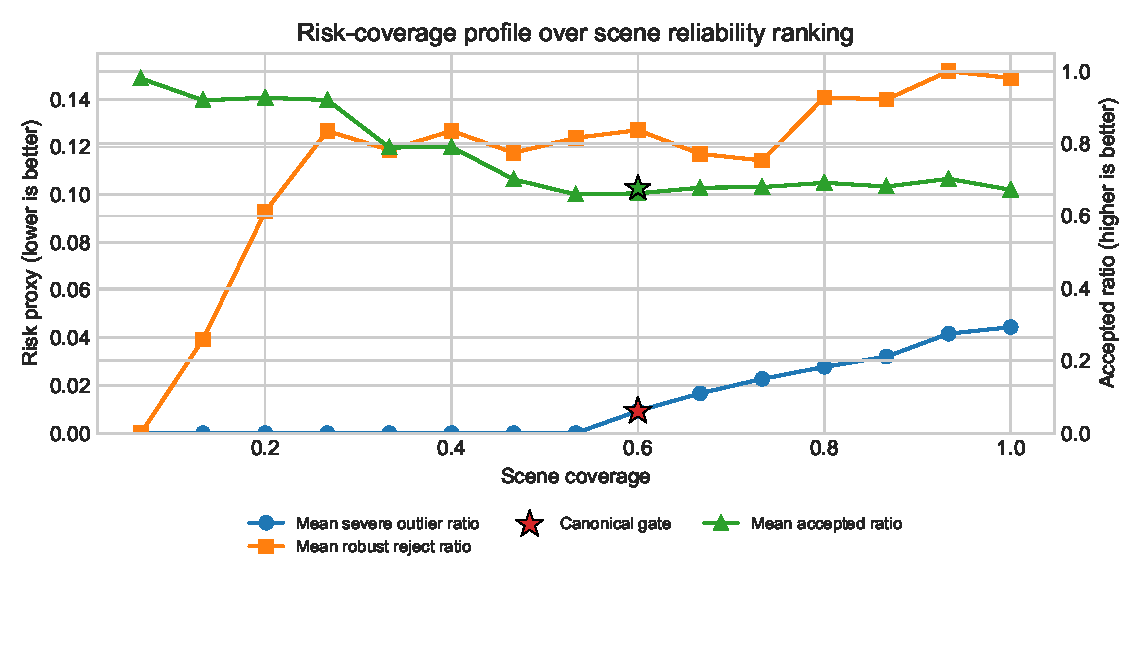
\includegraphics[width=0.82\textwidth]{figures/fig_risk_coverage_curve.pdf}
\caption{Risk-coverage operating profile on UAV-TAlign-12K. The curves are generated by ranking
scenes with the non-trained reliability score and progressively increasing retained coverage. The
star marks the strict canonical QA-gate operating point (9/15 retained scenes). The score-ranked
top-$K$ operating points visualize the reliability--coverage profile and do not replace the
canonical decision rule.}
\label{fig:risk_coverage}
\end{figure}

At the canonical point, UAV-TAlign retains 9 scenes, covers 60.0\% of scenes and 74.4\% of
evaluated pairs, and keeps the mean severe-outlier ratio at 0.009. The score-ranked curve exposes a
smooth operating profile from conservative high-confidence retention to broader inclusive
coverage. We keep the canonical gate fixed and use this curve to visualize the reliability--coverage
trade-off.

\subsection{Cumulative Ablation}

The accepted 8-scene supplement clarifies two complementary points. First, QA-aware verification
turns a permissive scene-pass pipeline into a retained-product decision rule. Second, the frame
selection policy matters primarily near the pass/fail boundary rather than through large changes
in overall accepted-frame support. On this subset, the candidate-only and consensus-only variants
both keep 8/8 scenes under the pre-verification criterion, whereas the deterministic-even
QA-aware variant contracts to 5/8 retained scenes.

\begin{table}[t]
\caption{Frozen cumulative ablation on the fixed 8-scene subset. The table emphasizes retained
product behavior under the accepted local supplement evidence.}
\label{tab:ablation_main}
\centering
\resizebox{\textwidth}{!}{
\begin{tabular}{lcccrrrr}
\toprule
Variant & Selection & Consensus & Verification & Retained/N $\uparrow$ & QA Pass/N $\uparrow$ & Acc. Mean $\uparrow$ & Acc. Range \\
\midrule
A1 candidate only & candidate-only & \xmark & \xmark & 8/8 & 5/8 & 13.6 & 8--34 \\
A2 + robust scene consensus & candidate-only & \cmark & \xmark & 8/8 & 5/8 & 13.6 & 8--34 \\
A3 + QA-aware verification & even & \cmark & \cmark & 5/8 & 5/8 & 26.0 & 7--49 \\
Random selection full (seed0) & random & \cmark & \cmark & 5/8 & 6/8 & 26.6 & 7--49 \\
\bottomrule
\end{tabular}}
\end{table}

The accepted random-selection supplement further shows a 5/8 to 7/8 spread across seeds on the
same fixed subset. The variation is concentrated in a small number of borderline scenes, while the
accepted-frame means remain comparatively stable across seeds. Deterministic-even selection
therefore serves as a reproducible default operating policy, and the multi-seed result is best
read as boundary sensitivity rather than full-pipeline instability.

\begin{figure}[t]
\centering
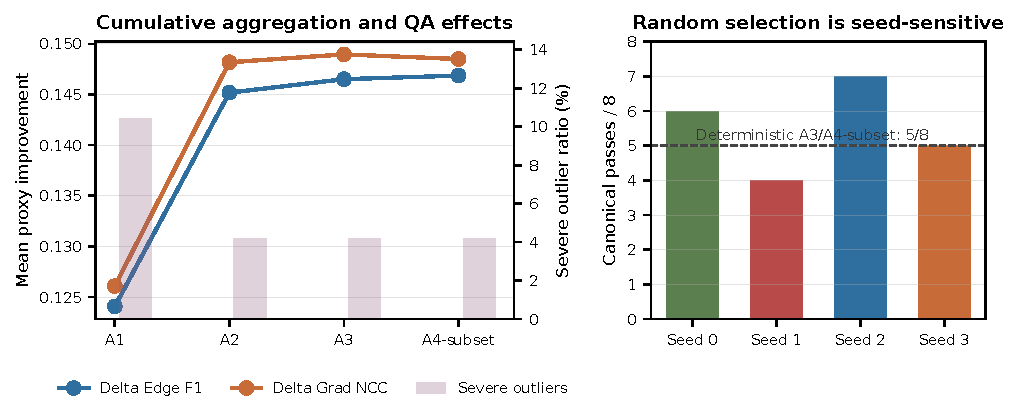
\includegraphics[width=\textwidth]{figures/fig_ablation_sensitivity.pdf}
\caption{Cumulative ablation and random-selection supplement. Robust scene consensus improves proxy
quality before the final gate, while the random-selection variant shows non-trivial seed
sensitivity on the same fixed 8-scene subset.}
\label{fig:ablation_sensitivity}
\end{figure}

% !TEX root = ../paper.tex

\section{Discussion}

\subsection{What UAV-TAlign-12K Reveals}

The main contribution of UAV-TAlign-12K is a captured dataset and protocol that expose a gap hidden
by pairwise-only reporting. Modern matchers provide abundant frame-level evidence on the official
split, yet the strict scene-level criterion retains only a subset of scenes. The benchmark
therefore separates two practically different capabilities: producing a pairwise homography and
deciding whether multi-frame evidence supports a trustworthy scene transform.

The protocol evidence supports this dataset-centered reliability framing. Retained and QA-filtered scenes show
structured differences in accepted ratio, severe outlier behavior, and baseline-relative QA
signals, indicating that the canonical criterion captures scene-level reliability beyond pairwise
matcher availability alone. This gives the evaluation a clear diagnostic role: it tests when
abundant pairwise evidence becomes a trustworthy scene-level transform. The canonical scene
criterion is therefore designed for conservative retention of scene transforms rather than for
maximizing unconditional scene acceptance.

UAV-TAlign serves as a reference implementation for this second evaluation unit. Its evidence
selection, robust consensus, and QA-aware verification demonstrate one reproducible way to convert
pairwise hypotheses into a retained scene product; the benchmark remains compatible with future
matchers and alternative scene-level aggregation strategies.

The multi-seed random-selection supplement further strengthens the design rationale for
deterministic evidence selection. On the accepted 8-scene subset, random selection spans 5/8 to
7/8 retained scenes across seeds, but the variation is concentrated in a few borderline scenes
rather than in large shifts of accepted-frame support. Deterministic-even selection therefore
provides a reproducible default operating policy, while robust scene consensus and QA-aware
verification define the retained-product decision layer.

\subsection{Scope, Limitations, and Intended Use}

UAV-TAlign-12K targets captured UAV scenes where a dominant planar or far-field transform is a
useful operating model. Its 15 scenes cover diverse illumination, thermal rendering, view, and
scene-family conditions, but they do not represent every flight altitude, sensor configuration, or
non-planar environment. The benchmark should therefore be interpreted as a focused resource for
cross-FOV homography alignment rather than a universal model of all UAV registration settings.

The label-free QA proxies enable scalable analysis without dense geometric annotations, but they
are scene-consistency diagnostics rather than substitutes for dense ground truth or downstream
task evaluation. The canonical gate is intentionally conservative, and the reliability score is
used only for ranking and coverage analysis. These boundaries make the protocol suitable for
comparing deployable scene-level reliability while leaving room for future annotations, geometric
models, and task-specific validation.

% !TEX root = ../paper.tex

\section{Conclusion}

This work reframes UAV infrared-visible registration from pairwise match availability to scene-level
alignment reliability. UAV-TAlign turns strong off-the-shelf multimodal matching into retained
scene-level decisions through reliability-guided evidence selection, robust scene consensus, and
QA-aware verification. Across formal evaluation, protocol-consistency analysis, and cumulative
module ablations, the evidence shows that the decisive step is transforming abundant frame-level
matches into trustworthy scene-level alignment products.

Together with UAV-TAlign-12K and the accompanying label-free evaluation setup, UAV-TAlign provides
a practical and reproducible foundation for studying when scene-level alignment is reliable enough
to retain in real UAV infrared-visible imagery.

\section*{Data Availability}

UAV-TAlign-12K, the official evaluation manifest, metadata, and evaluation scripts will be made
publicly available upon publication. The official evaluation split contains 6,037 integrity-checked
RGB-infrared pairs from a 6,039-pair collection. The manifest hash is provided for reproducibility.


\bibliographystyle{elsarticle-num}
\bibliography{references}

\end{document}
